\documentclass[11pt,a4paper]{article}
\usepackage[margin=2.5cm]{geometry}
\usepackage{graphicx}
\usepackage{amsmath}
\usepackage{booktabs}
\usepackage{array}
\usepackage{listings}
\usepackage{xcolor}
\usepackage{hyperref}
\usepackage{caption}
\usepackage{tikz}
\usetikzlibrary{shapes.geometric,arrows.meta,positioning}

\lstset{
  basicstyle=\ttfamily\small,
  breaklines=true,
  frame=single,
  numbers=left,
  numberstyle=\tiny,
  keywordstyle=\bfseries,
  commentstyle=\itshape,
  showstringspaces=false
}
\setlength{\parskip}{0.5em}
\setlength{\parindent}{0pt}
\setlength{\emergencystretch}{3em}
\hypersetup{colorlinks=true, linkcolor=blue, urlcolor=blue}

\begin{document}

% ---------------- Title page ----------------
\begin{titlepage}
\thispagestyle{empty}
\begin{center}

\includegraphics[width=0.28\textwidth]{college_logo.jpg}

\vspace{1.2cm}
{\Large\bfseries A Course End Project Report on}\\[0.4cm]
{\huge\bfseries Vehicle Rental Management System}\\[0.6cm]
{\large Object Oriented Programming through Java Laboratory}\\[1.2cm]
{\large Submitted by}\\[0.3cm]
{\large\bfseries A Vivek Reddy \quad 25881A05EP}\\[1.2cm]
{\large Course Facilitator}\\[0.3cm]
{\large\bfseries Mr. D. Ganesh}\\[0.3cm]
{\large Assistant Professor}\\[1.2cm]
{\large Department of Computer Science and Engineering}\\[0.3cm]
{\large Vardhaman College of Engineering, Hyderabad}\\[0.6cm]
{\large October 2026}

\vspace{0.8cm}
{\small No other team members are included in this report, as instructed.\\
Sole student for this submission: A Vivek Reddy (25881A05EP).}
\end{center}
\end{titlepage}

\tableofcontents
\newpage

% ---------------- Abstract ----------------
\section*{Abstract}
\addcontentsline{toc}{section}{Abstract}

In many small vehicle-rental businesses, bookings are still kept in a
notebook or a loosely maintained spreadsheet. When the record is kept
that way, a vehicle that is already out can be promised to another
customer, a returned vehicle can stay marked as rented, and a price
calculated by hand can be wrong. This project presents a Vehicle Rental
Management System developed in Java. The system is a desktop
application built with Java Swing that manages vehicles, customers and
rentals: an operator can add and remove vehicles, add customers, rent
an available vehicle for a number of days, and return it so that it
becomes available again. Rental cost is calculated exactly, as daily
rate multiplied by number of days, using \texttt{BigDecimal}
arithmetic rather than floating-point arithmetic. Data are saved to
plain CSV files under \texttt{data/} and reloaded on the next launch,
so no database server or external library is required.

The application was audited file by file before any change was made.
The baseline already compiled cleanly and passed all of its tests.
One genuine gap was found and fixed in this work: the service layer
already supported searching vehicles, but the Swing user interface did
not expose it, so a search bar was added to the Vehicles tab. After
that change the project was recompiled and retested: compilation
succeeded, all 12 dependency-free service tests passed, and the
graphical interface was launched under a virtual display, where it
started with its six seeded vehicles and three seeded customers and
reported ``Available: 6 / 6 vehicles'' with no errors.

\textit{Keywords:} Vehicle rental, Java Swing, desktop application,
CSV persistence, \texttt{BigDecimal}, software testing.

% ---------------- 1 Introduction ----------------
\section{Introduction}

A vehicle-rental business must answer three questions at any moment:
which vehicles are free, who has rented which vehicle, and how much
each booking costs. When those answers live in a notebook or a
spreadsheet, double-booking is easy, a returned vehicle may stay
marked as rented, and revenue figures may not reconcile. The
consequences are practical rather than theoretical: a customer is
promised a vehicle that is already out, or a booking total has to be
recalculated by hand.

The Vehicle Rental Management System developed in this project
automates that record-keeping for a small business. It maintains a
record of every vehicle, containing an id, brand, model, type
(Car / Bike / SUV / Van), year and daily rental rate, together with
whether the vehicle is available or rented. It maintains a record of
every customer, containing an id, name, phone number and driving
licence number. Using a window with three tabs --- Vehicles,
Customers and Rentals --- the operator can add a vehicle, remove an
available vehicle, add a customer, rent an available vehicle to an
existing customer for a number of days, and return a rental. Because
the rental rules are written once inside the service layer, the same
double-booking guard and the same pricing rule are applied correctly
and uniformly to every booking.

This project also serves as a practical application of programming in
Java. It uses classes and objects, encapsulation, collections
(\texttt{ArrayList}), exact decimal arithmetic with
\texttt{BigDecimal}, file handling with CSV files, exception handling,
and a graphical user interface built with Swing, which are core
topics of the Object Oriented Programming through Java Laboratory
course. The system is deliberately
single-user and dependency-free: one operator, one machine, no
network service and no database server to install or administer.
That scope matches the way the application is actually used in the
code, and its limits are stated plainly in Section~5.1 rather than
hidden.

% ---------------- 2 Literature Review ----------------
\section{Literature Review}

Textbooks on Java programming describe the language features used in
this project. Schildt explains classes, encapsulation and the
Collections Framework in detail, including the \texttt{ArrayList}
class used here to store vehicles, customers and rentals [1].
Balagurusamy presents the same concepts with simple,
student-oriented examples, including menu-driven programs and
exception handling with \texttt{try}--\texttt{catch} blocks [2].
Deitel and Deitel discuss case-study style application development
in Java, in which a real-world problem is divided into classes with
clear responsibilities [3]. The official Java Tutorials from Oracle
provide reference documentation for the Collections Framework, for
Swing components such as tables and tabbed panes, and for
\texttt{BigDecimal} arithmetic [4, 5].

On the application side, the same argument that applies to
computerising a payroll register applies to a rental register: when
a routine administrative process is moved from paper to a program,
the rules are written once instead of being re-applied by hand in
every row, so they cannot be changed accidentally in one entry, and
an invalid operation can be reported immediately instead of
silently producing a wrong record. Compared with a spreadsheet, a
program written in Java has two advantages for this problem. First,
the double-booking rule cannot be bypassed by editing a cell, because
it is enforced in the service layer before a rental is created.
Second, the program validates every booking --- unknown vehicle,
unknown customer, non-positive days, or a vehicle already rented ---
and reports the problem in an error dialogue instead of creating a
booking that contradicts the fleet record. The present project
follows that idea at a small scale: it computerises the vehicle,
customer and rental records and the pricing rule, but keeps the
rules simple and transparent so that every booking total can be
checked by hand, as daily rate multiplied by days.

% ---------------- 3 Objectives ----------------
\section{Objectives}

\begin{itemize}
  \item To develop a Java Swing Vehicle Rental Management System for
        maintaining vehicle, customer and rental records.
  \item To add, list, search and remove vehicles, and to add and list
        customers, using \texttt{ArrayList} collections.
  \item To rent an available vehicle to an existing customer for a
        positive number of days, and to prevent double-booking.
  \item To calculate the rental total automatically and exactly as
        daily rate $\times$ number of days, using \texttt{BigDecimal}.
  \item To return a rental, restoring the vehicle's availability, and
        to keep a record of both active and returned rentals.
  \item To persist vehicles, customers and rentals to CSV files and
        reload them on launch, seeding sample data only on a first
        run when no saved data exist.
  \item To keep the project dependency-free, so that it builds with
        a JDK alone, and to verify it by compilation, automated
        tests and a genuine graphical run.
\end{itemize}

% ---------------- 4 Methodology ----------------
\section{Methodology}

\subsection{Architectural Diagram}

The system follows a simple layered structure, as shown in
Figure~1. The operator interacts with the Swing window provided by
\texttt{RentalApp}. Each tab and button calls the service layer,
\texttt{RentalService}, which enforces the business rules. The
service works with the model classes and with the persistence layer,
\texttt{CsvRentalStore}, which reads and writes the three CSV files.
The user interface never writes a CSV file directly and never
decides whether a booking is legal; it asks the service, and the
service decides. That is why the service can be tested without a
display, which is exactly how the test class works.

\begin{figure}[h]
\centering
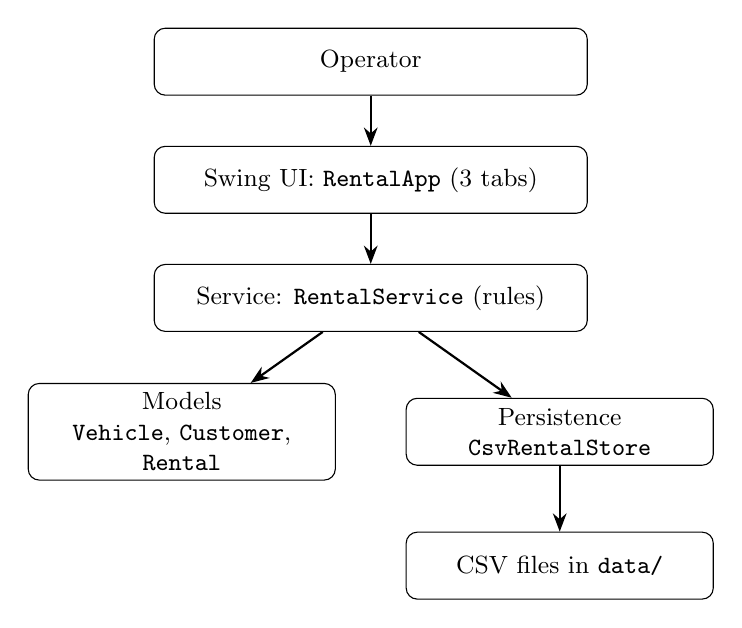
\begin{tikzpicture}[box/.style={draw, rounded corners, minimum width=5.5cm, minimum height=0.85cm, align=center, font=\small}, smallbox/.style={draw, rounded corners, minimum width=3.9cm, minimum height=0.85cm, align=center, font=\small}, arrow/.style={-Stealth, thick}]
\node[box] (op) at (0,3.0) {Operator};
\node[box] (ui) at (0,1.5) {Swing UI: \texttt{RentalApp} (3 tabs)};
\node[box] (svc) at (0,0) {Service: \texttt{RentalService} (rules)};
\node[smallbox] (model) at (-2.4,-1.7) {Models\\ \texttt{Vehicle}, \texttt{Customer},\\ \texttt{Rental}};
\node[smallbox] (store) at (2.4,-1.7) {Persistence\\ \texttt{CsvRentalStore}};
\node[smallbox] (csv) at (2.4,-3.4) {CSV files in \texttt{data/}};
\draw[arrow] (op) -- (ui);
\draw[arrow] (ui) -- (svc);
\draw[arrow] (svc) -- (model);
\draw[arrow] (svc) -- (store);
\draw[arrow] (store) -- (csv);
\end{tikzpicture}
\caption{Architectural diagram of the Vehicle Rental Management System.}
\end{figure}

On launch, \texttt{RentalApp.create()} tries to load saved data. If
no \texttt{vehicles.csv} exists it seeds sample data and saves it;
if loading fails it falls back to the same sample data so the
application still opens. The seeded fleet is V001 Maruti Swift
(Car, Rs.\ 1500/day), V002 Hyundai Creta (SUV, Rs.\ 2800/day),
V003 Honda Activa (Bike, Rs.\ 500/day), V004 Toyota Innova
(Van, Rs.\ 3500/day), V005 Royal Enfield Classic 350 (Bike,
Rs.\ 900/day) and V006 Tata Nexon (SUV, Rs.\ 2600/day), together
with customers C001, C002 and C003. These are sample records in the
code, not records of real rentals.

\subsection{Hardware and Software Requirements}

\begin{itemize}
  \item Processor: Any modern processor (Intel Core i3 or equivalent
        and above).
  \item RAM: 4 GB or more.
  \item Operating System: Windows / Linux / macOS (any system that
        supports the Java Development Kit and a graphical display).
  \item Java Development Kit (JDK): Version 17 or later (the program
        was compiled and tested with OpenJDK 17).
  \item Editor / IDE: Any text editor or IDE such as VS Code,
        IntelliJ IDEA or Eclipse.
  \item No other dependencies: no Maven, Gradle, database server or
        third-party library is required.
\end{itemize}

\subsection{Working Principle}

\begin{enumerate}
  \item The program starts by loading saved data, or by seeding the
        six sample vehicles and three sample customers described
        above when no saved data exist, so that the tabs can be used
        immediately.
  \item The main window shows three tabs: Vehicles, Customers and
        Rentals. The footer shows the total booked amount and the
        count of available vehicles, and a Save Data button writes
        the current state to \texttt{data/}.
  \item For adding a vehicle, the program reads the id, brand, model,
        type, year and daily rate. The year must lie between 1990
        and 2100 and the daily rate must be positive; otherwise the
        record is rejected with an error message. Duplicate vehicle
        and customer ids are rejected.
  \item For renting, the operator enters a vehicle id, a customer id
        and a number of days. The service rejects unknown ids, a
        non-positive number of days, and a vehicle that is already
        rented, then computes the total and creates an active
        rental dated today, marking the vehicle unavailable.
  \item For returning, the operator enters the rental id. The service
        rejects an unknown id and a rental that has already been
        returned, sets its status to \texttt{RETURNED}, and marks
        the vehicle available again.
  \item For searching, the operator types a keyword on the Vehicles
        tab. The search is a case-insensitive substring match over
        id, brand, model and type; Show All restores the full list.
  \item Removing a vehicle succeeds only if the vehicle exists and
        is available, so a vehicle that is out on rent can never be
        deleted from under an active booking.
  \item Add, rent and return actions save the data quietly after
        each successful change, and the tables and footer totals are
        refreshed.
\end{enumerate}

The rental rules used in this project are summarised in Table~1.

\begin{table}[h]
\centering
\caption{Rental rules}
\begin{tabular}{ll}
\toprule
Rule & Statement \\
\midrule
Rental total & Daily rate $\times$ number of days (\texttt{BigDecimal}) \\
Days & Must be positive \\
Availability & A vehicle can be rented only when available \\
Double-booking & An already rented vehicle cannot be rented again \\
Return & Restores availability; status becomes \texttt{RETURNED} \\
Removal & Only an available vehicle can be removed \\
Search & Id, brand, model or type, case-insensitive \\
Total booked & Sum of all rental totals, active and returned \\
\bottomrule
\end{tabular}
\end{table}

\subsection{Software Implementation}

The program is written in Java using seven application source files.
\texttt{Main.java} is the entry point and launches the Swing UI on
the event-dispatch thread. \texttt{model/Vehicle.java},
\texttt{model/Customer.java} and \texttt{model/Rental.java} hold
the data, with validation in their constructors. \texttt{service/}
\texttt{RentalService.java} contains all business rules: add,
search, rent, return, totals and sample data. \texttt{persistence/}
\texttt{CsvRentalStore.java} saves and loads the three CSV files.
\texttt{ui/RentalApp.java} provides the three-tab Swing window,
input dialogues, error dialogues, footer totals and the Save button.
The complete source is included in the source package submitted with
this report. The central booking method, which contains the
double-booking guard and the pricing rule, is given below.

\begin{lstlisting}[caption={RentalService.rentVehicle -- the central booking method}]
public Rental rentVehicle(String vehicleId, String customerId, int days) {
    Vehicle vehicle = findVehicle(vehicleId)
            .orElseThrow(() -> new IllegalArgumentException("No such vehicle: " + vehicleId));
    findCustomer(customerId)
            .orElseThrow(() -> new IllegalArgumentException("No such customer: " + customerId));
    if (days <= 0) {
        throw new IllegalArgumentException("days must be positive");
    }
    if (!vehicle.isAvailable()) {
        throw new IllegalStateException("Vehicle is already rented: " + vehicleId);
    }
    BigDecimal total = vehicle.getDailyRate().multiply(BigDecimal.valueOf(days));
    Rental rental = new Rental(nextRentalId(), vehicleId, customerId, days,
            total, LocalDate.now(), Rental.Status.ACTIVE);
    rentals.add(rental);
    vehicle.setAvailable(false);
    return rental;
}
\end{lstlisting}

The important implementation details are:

\begin{itemize}
  \item \textbf{Separation of concerns:} The UI, the service, the
        models and the store are separate, so the service can be
        tested without a display.
  \item \textbf{Exact money arithmetic:} Daily rates and totals are
        \texttt{BigDecimal}, never floating-point, so a total such
        as Rs.\ 1500 $\times$ 3 is exactly Rs.\ 4500.
  \item \textbf{Collections:} Vehicles, customers and rentals are
        held in \texttt{ArrayList} collections, and the service
        returns copies of its lists so callers cannot accidentally
        mutate its internal state.
  \item \textbf{Validation:} Vehicle construction rejects a year
        outside 1990--2100 and a non-positive rate; rental
        construction rejects non-positive days; duplicate ids are
        rejected.
  \item \textbf{Exception handling:} Invalid operations throw
        \texttt{IllegalArgumentException} or
        \texttt{IllegalStateException}, and the UI shows the
        exception's message in an error dialogue instead of
        crashing or creating a contradictory record.
  \item \textbf{Persistence:} \texttt{CsvRentalStore.save} writes
        one line per record to each CSV file, replacing commas
        inside text fields with spaces so that a plain split on
        commas is safe on load. Rental ids are generated
        sequentially as R001, R002, and so on, and loading advances
        the sequence past any loaded id so that a new rental cannot
        collide with a reloaded one.
  \item \textbf{Change made in this work:} Inspection found that
        \texttt{searchVehicles} existed and was tested, but no
        control in the Swing window called it, while the README
        described search as a feature. A search bar was therefore
        added to the Vehicles tab, with a Search button that
        refreshes the vehicle table with
        \texttt{service.searchVehicles(text)} and a Show All button
        that restores the full list, sharing the same table-refresh
        code. No other behaviour was changed.
\end{itemize}

% ---------------- 5 Results and Discussion ----------------
\section{Results and Discussion}

The program was compiled with \texttt{javac --release 17}
(OpenJDK 17) with no errors, using \texttt{./compile.sh}, and was
tested with the dependency-free test class
\texttt{RentalServiceTest}, run via \texttt{./test.sh}. In total,
12 test cases were executed and all 12 passed. The test cases are
listed in Table~2.

\begin{table}[h]
\centering
\caption{Test cases and results}
\begin{tabular}{ll}
\toprule
No. & Test case and result \\
\midrule
1 & Rent cost: Rs.\ 1500 $\times$ 3 days = Rs.\ 4500 --- Passed \\
2 & Rented vehicle becomes unavailable --- Passed \\
3 & One vehicle still available after one rental --- Passed \\
4 & Double booking rejected --- Passed \\
5 & Returned vehicle available again --- Passed \\
6 & Re-rent cost: Rs.\ 1500 $\times$ 2 days = Rs.\ 3000 --- Passed \\
7 & Search by model finds Swift --- Passed \\
8 & Search by type finds Bike --- Passed \\
9 & Duplicate vehicle id rejected --- Passed \\
10 & Rented vehicle cannot be removed --- Passed \\
11 & Available vehicle can be removed --- Passed \\
12 & Unknown vehicle id rejected --- Passed \\
\bottomrule
\end{tabular}
\end{table}

The booking total was verified by hand. For the Swift at
Rs.\ 1500 per day rented for 3 days: $1500 \times 3 = 4500$.
After return and re-rent for 2 days: $1500 \times 2 = 3000$.
Both values match the program output exactly. The graphical
application was then launched under a virtual display (Xvfb) from
a clean copy, so that its first-launch path was exercised. It
created \texttt{data/vehicles.csv} (6 lines),
\texttt{data/customers.csv} (3 lines) and
\texttt{data/rentals.csv} (empty, as no rental had yet been made),
matching the seeded data in Section~4.1, and it ran with no errors
until it was stopped. A screenshot taken during that run is shown
in Figure~2.

\begin{figure}[h]
\centering
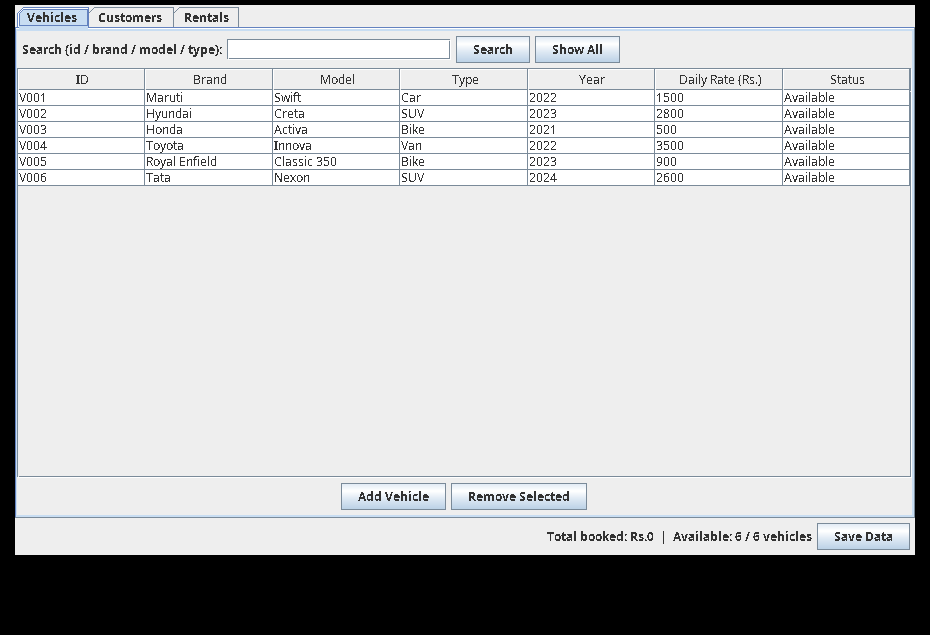
\includegraphics[width=\textwidth]{vehicle-main.png}
\caption{Main window of the Vehicle Rental Management System on first launch: Vehicles tab, search bar, seeded fleet, and footer totals. Captured from the actual running application, not drawn or mocked.}
\end{figure}

From these results, the system meets its objectives: vehicle,
customer and rental records are maintained correctly, the pricing
rule is accurate and uniform for every booking, double-booking is
prevented, and invalid inputs are handled without the program
stopping. No performance measurement is claimed: the application
is a small desktop tool, no benchmark was run, and no timing or
throughput figure appears in this report.

\subsection{Limitations and Future Enhancements}

The present system is single-user, so there is no login, no
concurrency control and no file locking; two copies writing the
same CSV files could overwrite each other. A rental records a
start date and a number of days, but there is no calendar check
for overlapping future bookings --- availability is simply ``free
now or rented now''. Totals are booked amounts only; payment,
deposit, late-return and damage charges are not modelled. The
plain CSV store replaces commas in text fields with spaces on
save, has no backup or transaction, and a hand-edited malformed
CSV line can fail loading. Phone and licence formats are not
validated, and vehicles and customers can be added and (for
available vehicles) removed, but not edited in place from the UI.

In the future, the system can be improved by editing vehicle and
customer records, by a proper CSV escaping scheme or a small
embedded database, by date-range availability with a return date,
and only then by multi-user or web access, which would change the
architecture rather than extend it. Each of those is future work,
not a feature claimed here.

% ---------------- 6 Mapping POs and SDGs ----------------
\section{Mapping POs and SDGs}

\subsection{Program Outcomes (POs) Mapping}

\begin{table}[h]
\centering
\caption{Mapping of Program Outcomes (POs) to project relevance}
\begin{tabular}{p{1.2cm}p{4.2cm}p{8.6cm}}
\toprule
PO No. & Program Outcome & Relevance \\
\midrule
PO1 & Engineering Knowledge & Applied Java programming, data structures (\texttt{ArrayList}), \texttt{BigDecimal} arithmetic and file handling to a real rental-management problem. \\
PO2 & Problem Analysis & Analysed the manual rental register and identified where double-booking, stale availability and hand-calculated totals cause errors. \\
PO3 & Design / Development of Solutions & Designed a layered class structure (UI, service, models, store) and developed a working, persistent solution. \\
PO5 & Modern Tool Usage & Used JDK 17, the Swing framework and a modern code editor to build and test the application. \\
PO6 & Engineer and Society & Provides a clear, priced rental record, which is a practical requirement of a rental business and a basis of trust with its customers. \\
\bottomrule
\end{tabular}
\end{table}

\subsection{Sustainable Development Goals (SDGs) Mapping}

\begin{table}[h]
\centering
\caption{Mapping of Sustainable Development Goals (SDGs) to project relevance}
\begin{tabular}{p{1.4cm}p{4.2cm}p{8.4cm}}
\toprule
SDG No. & Goal & Relevance \\
\midrule
SDG 9 & Industry, Innovation and Infrastructure & Promotes the digitisation of a routine administrative process in a small business, replacing a paper register with a persistent program. \\
SDG 11 & Sustainable Cities and Communities & A well-run rental fleet makes shared use of existing vehicles easier to manage, so fewer vehicles need to be owned for occasional use. \\
SDG 12 & Responsible Consumption and Production & Keeping an accurate fleet and booking record supports efficient use of the vehicles already owned, rather than over-provisioning the fleet. \\
\bottomrule
\end{tabular}
\end{table}

% ---------------- 7 Conclusion ----------------
\section{Conclusion}

This project successfully implements a Vehicle Rental Management
System in Java. The system maintains vehicle, customer and rental
records, prices bookings exactly as daily rate multiplied by days,
prevents double-booking, restores availability on return, and
persists its data to CSV files, all through a simple three-tab
Swing interface. All 12 test cases passed, the booking totals were
verified by hand calculation, and a genuine graphical run with
seeded data and a captured screenshot confirmed that the
application starts and behaves as described. The project
demonstrates the practical use of classes, encapsulation,
collections, exact decimal arithmetic, file handling and exception
handling in solving a real administrative problem. Future
improvements in editing, date-range availability, a stronger
persistence format and, later, multi-user access can make the
system suitable for direct use in a larger rental business.

% ---------------- Bibliography ----------------
\begin{thebibliography}{9}
\addcontentsline{toc}{section}{Bibliography}

\bibitem{schildt} H. Schildt, \emph{Java: The Complete Reference},
12th ed., McGraw Hill, 2021.

\bibitem{balagurusamy} E. Balagurusamy, \emph{Programming with Java},
6th ed., McGraw Hill Education, 2019.

\bibitem{deitel} P. Deitel and H. Deitel, \emph{Java How to Program,
Early Objects}, 11th ed., Pearson, 2018.

\bibitem{oracle} Oracle, ``The Java Tutorials -- Collections, Swing
and Exception Handling,'' Oracle Corporation. [Online]. Available:
\url{https://docs.oracle.com/javase/tutorial/}

\bibitem{bigdecimal} Oracle, ``\texttt{java.math.BigDecimal} API
documentation,'' Oracle Corporation. [Online]. Available:
\url{https://docs.oracle.com/javase/17/docs/api/java.base/java/math/BigDecimal.html}

\end{thebibliography}

\end{document}
